% Options for packages loaded elsewhere
\PassOptionsToPackage{unicode}{hyperref}
\PassOptionsToPackage{hyphens}{url}
%
\documentclass[
]{article}
\title{Get and summarize AFSC survey data}
\author{Kirstin Holsman, Alaska Fisheries Science Center}
\date{}

\usepackage{amsmath,amssymb}
\usepackage{lmodern}
\usepackage{iftex}
\ifPDFTeX
  \usepackage[T1]{fontenc}
  \usepackage[utf8]{inputenc}
  \usepackage{textcomp} % provide euro and other symbols
\else % if luatex or xetex
  \usepackage{unicode-math}
  \defaultfontfeatures{Scale=MatchLowercase}
  \defaultfontfeatures[\rmfamily]{Ligatures=TeX,Scale=1}
\fi
% Use upquote if available, for straight quotes in verbatim environments
\IfFileExists{upquote.sty}{\usepackage{upquote}}{}
\IfFileExists{microtype.sty}{% use microtype if available
  \usepackage[]{microtype}
  \UseMicrotypeSet[protrusion]{basicmath} % disable protrusion for tt fonts
}{}
\makeatletter
\@ifundefined{KOMAClassName}{% if non-KOMA class
  \IfFileExists{parskip.sty}{%
    \usepackage{parskip}
  }{% else
    \setlength{\parindent}{0pt}
    \setlength{\parskip}{6pt plus 2pt minus 1pt}}
}{% if KOMA class
  \KOMAoptions{parskip=half}}
\makeatother
\usepackage{xcolor}
\IfFileExists{xurl.sty}{\usepackage{xurl}}{} % add URL line breaks if available
\IfFileExists{bookmark.sty}{\usepackage{bookmark}}{\usepackage{hyperref}}
\hypersetup{
  pdftitle={Get and summarize AFSC survey data},
  pdfauthor={Kirstin Holsman, Alaska Fisheries Science Center},
  hidelinks,
  pdfcreator={LaTeX via pandoc}}
\urlstyle{same} % disable monospaced font for URLs
\usepackage[margin=1in]{geometry}
\usepackage{color}
\usepackage{fancyvrb}
\newcommand{\VerbBar}{|}
\newcommand{\VERB}{\Verb[commandchars=\\\{\}]}
\DefineVerbatimEnvironment{Highlighting}{Verbatim}{commandchars=\\\{\}}
% Add ',fontsize=\small' for more characters per line
\usepackage{framed}
\definecolor{shadecolor}{RGB}{248,248,248}
\newenvironment{Shaded}{\begin{snugshade}}{\end{snugshade}}
\newcommand{\AlertTok}[1]{\textcolor[rgb]{0.94,0.16,0.16}{#1}}
\newcommand{\AnnotationTok}[1]{\textcolor[rgb]{0.56,0.35,0.01}{\textbf{\textit{#1}}}}
\newcommand{\AttributeTok}[1]{\textcolor[rgb]{0.77,0.63,0.00}{#1}}
\newcommand{\BaseNTok}[1]{\textcolor[rgb]{0.00,0.00,0.81}{#1}}
\newcommand{\BuiltInTok}[1]{#1}
\newcommand{\CharTok}[1]{\textcolor[rgb]{0.31,0.60,0.02}{#1}}
\newcommand{\CommentTok}[1]{\textcolor[rgb]{0.56,0.35,0.01}{\textit{#1}}}
\newcommand{\CommentVarTok}[1]{\textcolor[rgb]{0.56,0.35,0.01}{\textbf{\textit{#1}}}}
\newcommand{\ConstantTok}[1]{\textcolor[rgb]{0.00,0.00,0.00}{#1}}
\newcommand{\ControlFlowTok}[1]{\textcolor[rgb]{0.13,0.29,0.53}{\textbf{#1}}}
\newcommand{\DataTypeTok}[1]{\textcolor[rgb]{0.13,0.29,0.53}{#1}}
\newcommand{\DecValTok}[1]{\textcolor[rgb]{0.00,0.00,0.81}{#1}}
\newcommand{\DocumentationTok}[1]{\textcolor[rgb]{0.56,0.35,0.01}{\textbf{\textit{#1}}}}
\newcommand{\ErrorTok}[1]{\textcolor[rgb]{0.64,0.00,0.00}{\textbf{#1}}}
\newcommand{\ExtensionTok}[1]{#1}
\newcommand{\FloatTok}[1]{\textcolor[rgb]{0.00,0.00,0.81}{#1}}
\newcommand{\FunctionTok}[1]{\textcolor[rgb]{0.00,0.00,0.00}{#1}}
\newcommand{\ImportTok}[1]{#1}
\newcommand{\InformationTok}[1]{\textcolor[rgb]{0.56,0.35,0.01}{\textbf{\textit{#1}}}}
\newcommand{\KeywordTok}[1]{\textcolor[rgb]{0.13,0.29,0.53}{\textbf{#1}}}
\newcommand{\NormalTok}[1]{#1}
\newcommand{\OperatorTok}[1]{\textcolor[rgb]{0.81,0.36,0.00}{\textbf{#1}}}
\newcommand{\OtherTok}[1]{\textcolor[rgb]{0.56,0.35,0.01}{#1}}
\newcommand{\PreprocessorTok}[1]{\textcolor[rgb]{0.56,0.35,0.01}{\textit{#1}}}
\newcommand{\RegionMarkerTok}[1]{#1}
\newcommand{\SpecialCharTok}[1]{\textcolor[rgb]{0.00,0.00,0.00}{#1}}
\newcommand{\SpecialStringTok}[1]{\textcolor[rgb]{0.31,0.60,0.02}{#1}}
\newcommand{\StringTok}[1]{\textcolor[rgb]{0.31,0.60,0.02}{#1}}
\newcommand{\VariableTok}[1]{\textcolor[rgb]{0.00,0.00,0.00}{#1}}
\newcommand{\VerbatimStringTok}[1]{\textcolor[rgb]{0.31,0.60,0.02}{#1}}
\newcommand{\WarningTok}[1]{\textcolor[rgb]{0.56,0.35,0.01}{\textbf{\textit{#1}}}}
\usepackage{graphicx}
\makeatletter
\def\maxwidth{\ifdim\Gin@nat@width>\linewidth\linewidth\else\Gin@nat@width\fi}
\def\maxheight{\ifdim\Gin@nat@height>\textheight\textheight\else\Gin@nat@height\fi}
\makeatother
% Scale images if necessary, so that they will not overflow the page
% margins by default, and it is still possible to overwrite the defaults
% using explicit options in \includegraphics[width, height, ...]{}
\setkeys{Gin}{width=\maxwidth,height=\maxheight,keepaspectratio}
% Set default figure placement to htbp
\makeatletter
\def\fps@figure{htbp}
\makeatother
\setlength{\emergencystretch}{3em} % prevent overfull lines
\providecommand{\tightlist}{%
  \setlength{\itemsep}{0pt}\setlength{\parskip}{0pt}}
\setcounter{secnumdepth}{-\maxdimen} % remove section numbering
\ifLuaTeX
  \usepackage{selnolig}  % disable illegal ligatures
\fi

\begin{document}
\maketitle

{
\setcounter{tocdepth}{2}
\tableofcontents
}
\hypertarget{afsc-survey-cpue-data-github.comkholsmanafsc_cpue}{%
\paragraph{\texorpdfstring{\href{https://github.com/kholsman/AFSC_CPUE}{\textbf{AFSC
Survey CPUE data:
github.com/kholsman/AFSC\_CPUE}}}{AFSC Survey CPUE data: github.com/kholsman/AFSC\_CPUE}}\label{afsc-survey-cpue-data-github.comkholsmanafsc_cpue}}

Repo maintained by:\\
Kirstin Holsman\\
Alaska Fisheries Science Center\\
NOAA Fisheries, Seattle WA\\
\textbf{\url{kirstin.holsman@noaa.gov}}\strut \\
\emph{Last updated: Mar 03, 2023}

\hypertarget{overview}{%
\section{Overview}\label{overview}}

The below scripts return a list object cpue\_data saved as a compressed
Rdata file with the naming `reg.srvy\#.spp.cpue\_data.Rdata' such as
``ebs.srvy98.plk.cpue\_data.Rdata''. Each cpue\_data list contains 8
data.frames:

\begin{Shaded}
\begin{Highlighting}[]
\FunctionTok{load}\NormalTok{(}\FunctionTok{paste0}\NormalTok{(}\StringTok{"data/out/"}\NormalTok{,qrydate,}\StringTok{"/cpue/ebs/ebs.srvy98.plk.cpue\_data.Rdata"}\NormalTok{))}

\FunctionTok{names}\NormalTok{(cpue\_data)}
\end{Highlighting}
\end{Shaded}

There is a folder for each region ``ebs'', ``goa'', ``ai''. For the
``ebs'' (Bering Sea) there are two sets of cpue\_data, one that is
NEBS+SEBS combined (`ebs.srvy98.{[}sp{]}.cpue\_data.Rdata') and one that
is just SEBS survey areas (`sebs.srvy98.{[}sp{]}.cpue\_data.Rdata'). For
both the Gulf of Alaska (``goa'') and the Bering Sea, mean CPUE (Kg per
km2 or Number per km2) for each size bin at each strata was calculated
and then multiplied by the STRATA area to get total Biomass and
abundance. \textbf{Note:Since strata area estimates where not available
for the Aleutian Island (``ai'') or slope surveys (``slope'') these AREA
was set equal to 1 and the Total Biomass and abundance is actually the
sum of mean biomass. }

The data.frames within each cpue\_data object are:

\begin{enumerate}
\def\labelenumi{\arabic{enumi}.}
\tightlist
\item
  \textbf{totalB\_N}: Total biomass (kg) or abundance (\# of fish) for
  the species in each year\\
\item
  \textbf{mnCPUE\_strata\_yr} : Average survey CPUE (kg per Km2) or
  abundance (\# per Km2) for the species in each strata and year\\
\item
  \textbf{total\_bin\_B\_N}: Total biomass (kg) or abundance (\# of
  fish) for each bin (10 mm) for the species in each year\\
\item
  \textbf{mnCPUE\_strata\_bin\_yr} : Average survey CPUE (kg per Km2) or
  abundance (\# per Km2) for each size bin for the species in each
  strata and year
\item
  \textbf{CPUE\_station\_bin\_yr}: Station specific survey CPUE (kg per
  Km2) or abundance (\# per Km2) for each size bin for the species in
  each year\\
\item
  \textbf{CPUE\_station\_yr}: Station specific survey CPUE (kg per Km2)
  or abundance (\# per Km2) for the species in each year\\
\item
  \textbf{propByBin}: proportion of biomass in each size bin per species
  per year\\
\item
  \textbf{propByStrata}: proportion of biomass in each strata per
  species per year
\item
  \textbf{propByStrataBin}: proportion of biomass in each bin and strata
  per species per year
\end{enumerate}

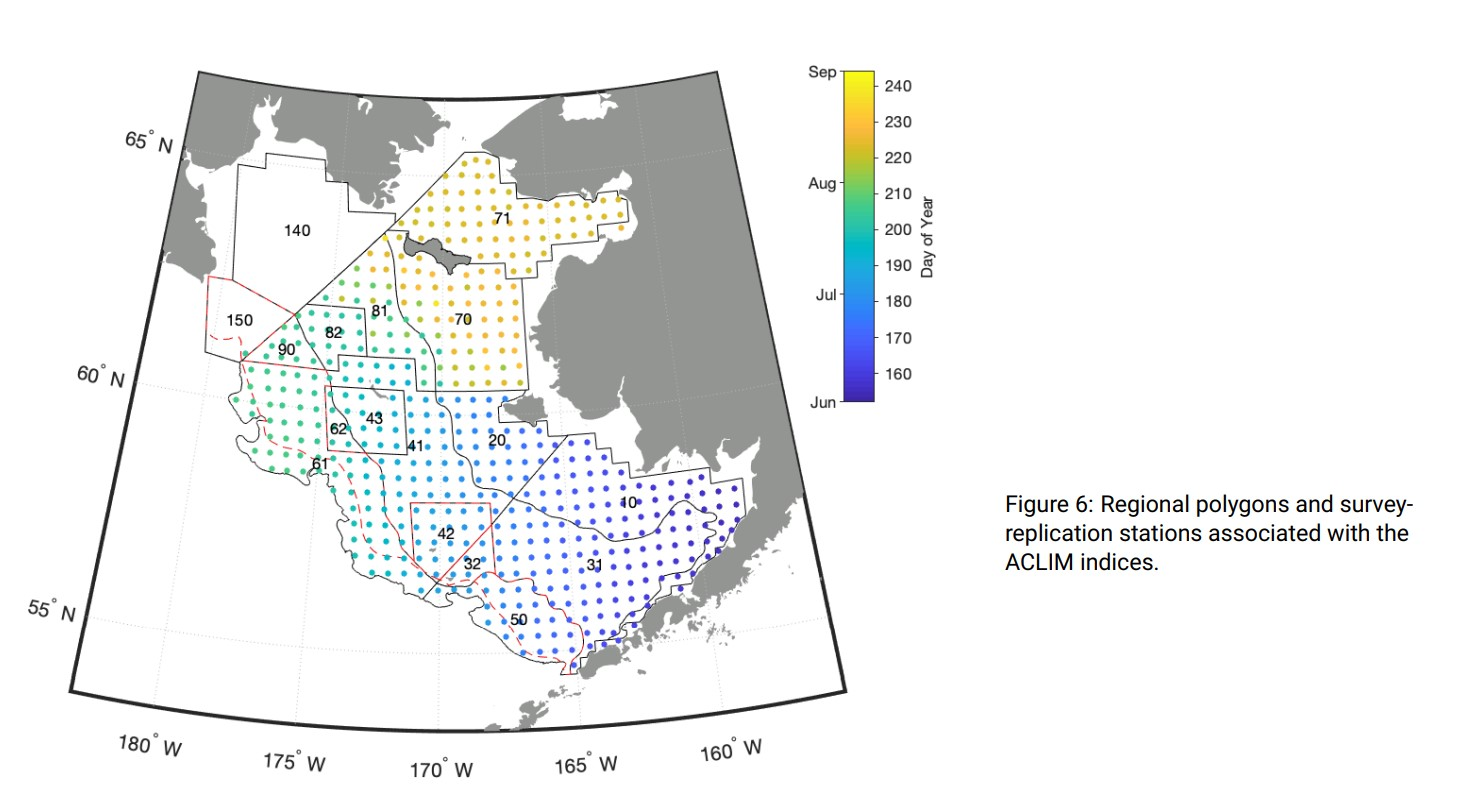
\includegraphics{figs/Kearney_2023.jpg} These are calculated from the
RACEBASE data tables for survey results where total CPUE was recorded
for the species \(s\) (location\_catch) at each haul, expanded to
include stations \(i\) where CPUE=0 (location) and expanded to each size
bin \(l\) using the proportional subset of frequency of fish of given
length (mm), binned into 10 mm bins (\(l\)) and predicted weight
(\(\hat{W}\)) for each size bin \(l\) at each station \(i\):

\[B_{s,y} =  \bar{CPUE_{s,k,y}} \dot{}A_{k}\] where \(A_{k}\) is the
area of the strata \(k\) in \(Km^2\) and \(\bar{CPUE_{s,k,y}}\) is the
strata specific average CPUE (kg per \(Km^2\) or number per \(Km^2\)) of
all stations \(i\) in strata \(k\):
\[\bar{CPUE_{s,k,y}} = \frac{1}{n_k}\dot{}\sum_{n_k}{CPUE_{s,k,y,i}}\]
where \$ CPUE\_\{s,k,y,i\} \$ is the station specific CPUE (saves as the
object \texttt{cpue\_data\$CPUE\_station\_yr}).

To obtain population level estimates of the biomass or abundance of fish
by size bin \(l\), we used a length weight regression to esimate the
weight of each size fish \(j\) measured (\(\hat{W}\)) to calculate the
proportion by weight or frequency at each station where
\[\hat{W} = \alpha_s+L_j^{\beta_s} \] where \(\alpha_s\) and \(\beta_s\)
are fit (updated each year) to all available length and weight data from
surveys from all years across the EBS, GOA, and AI (rather than each
basin separately) and
\[p^w_{l,i} = \frac{N_{l,i}\dot{}\hat{\bar{W_{l,i}}}}{\sum_{}{N_{l,i}\dot{}\hat{\bar{W_{l,i}}}}}\]
and \[p^N_{l,i} = \frac{N_{l,i}}{\sum_{}{N_{l,i}}}\] This was then
multiplied by the CPUE at each station (\(CPUE_{s,k,y,i}\)) to obtain a
station estimate of CPUE by size bin \(l\)
\[CPUE_{s,k,y,l,i} = p^N_{l,i}\dot{}CPUE_{s,k,y,i}\]

Finally, the average strata CPUE (\(\bar{CPUE_{s,k,y,l}}\)) and whole of
EBS biomass by size bin (\(B_{s,y,l}\)) was calculated as:
\[\bar{CPUE_{s,k,y,l}} = \frac{1}{n_k}\dot{}\sum_{n_k}{CPUE_{s,k,y,l,i}}\]
and
\[B_{s,y,l}= \frac{\bar{CPUE_{s,k,y,l}}\dot{}A_{k}}{\sum_{n_k}{\bar{CPUE_{s,k,y,l}}\dot{}A_{k}}}\dot{}B_{s,y}\]

\hypertarget{comparison-of-bering-sea-survey-values}{%
\section{Comparison of Bering Sea survey
values}\label{comparison-of-bering-sea-survey-values}}

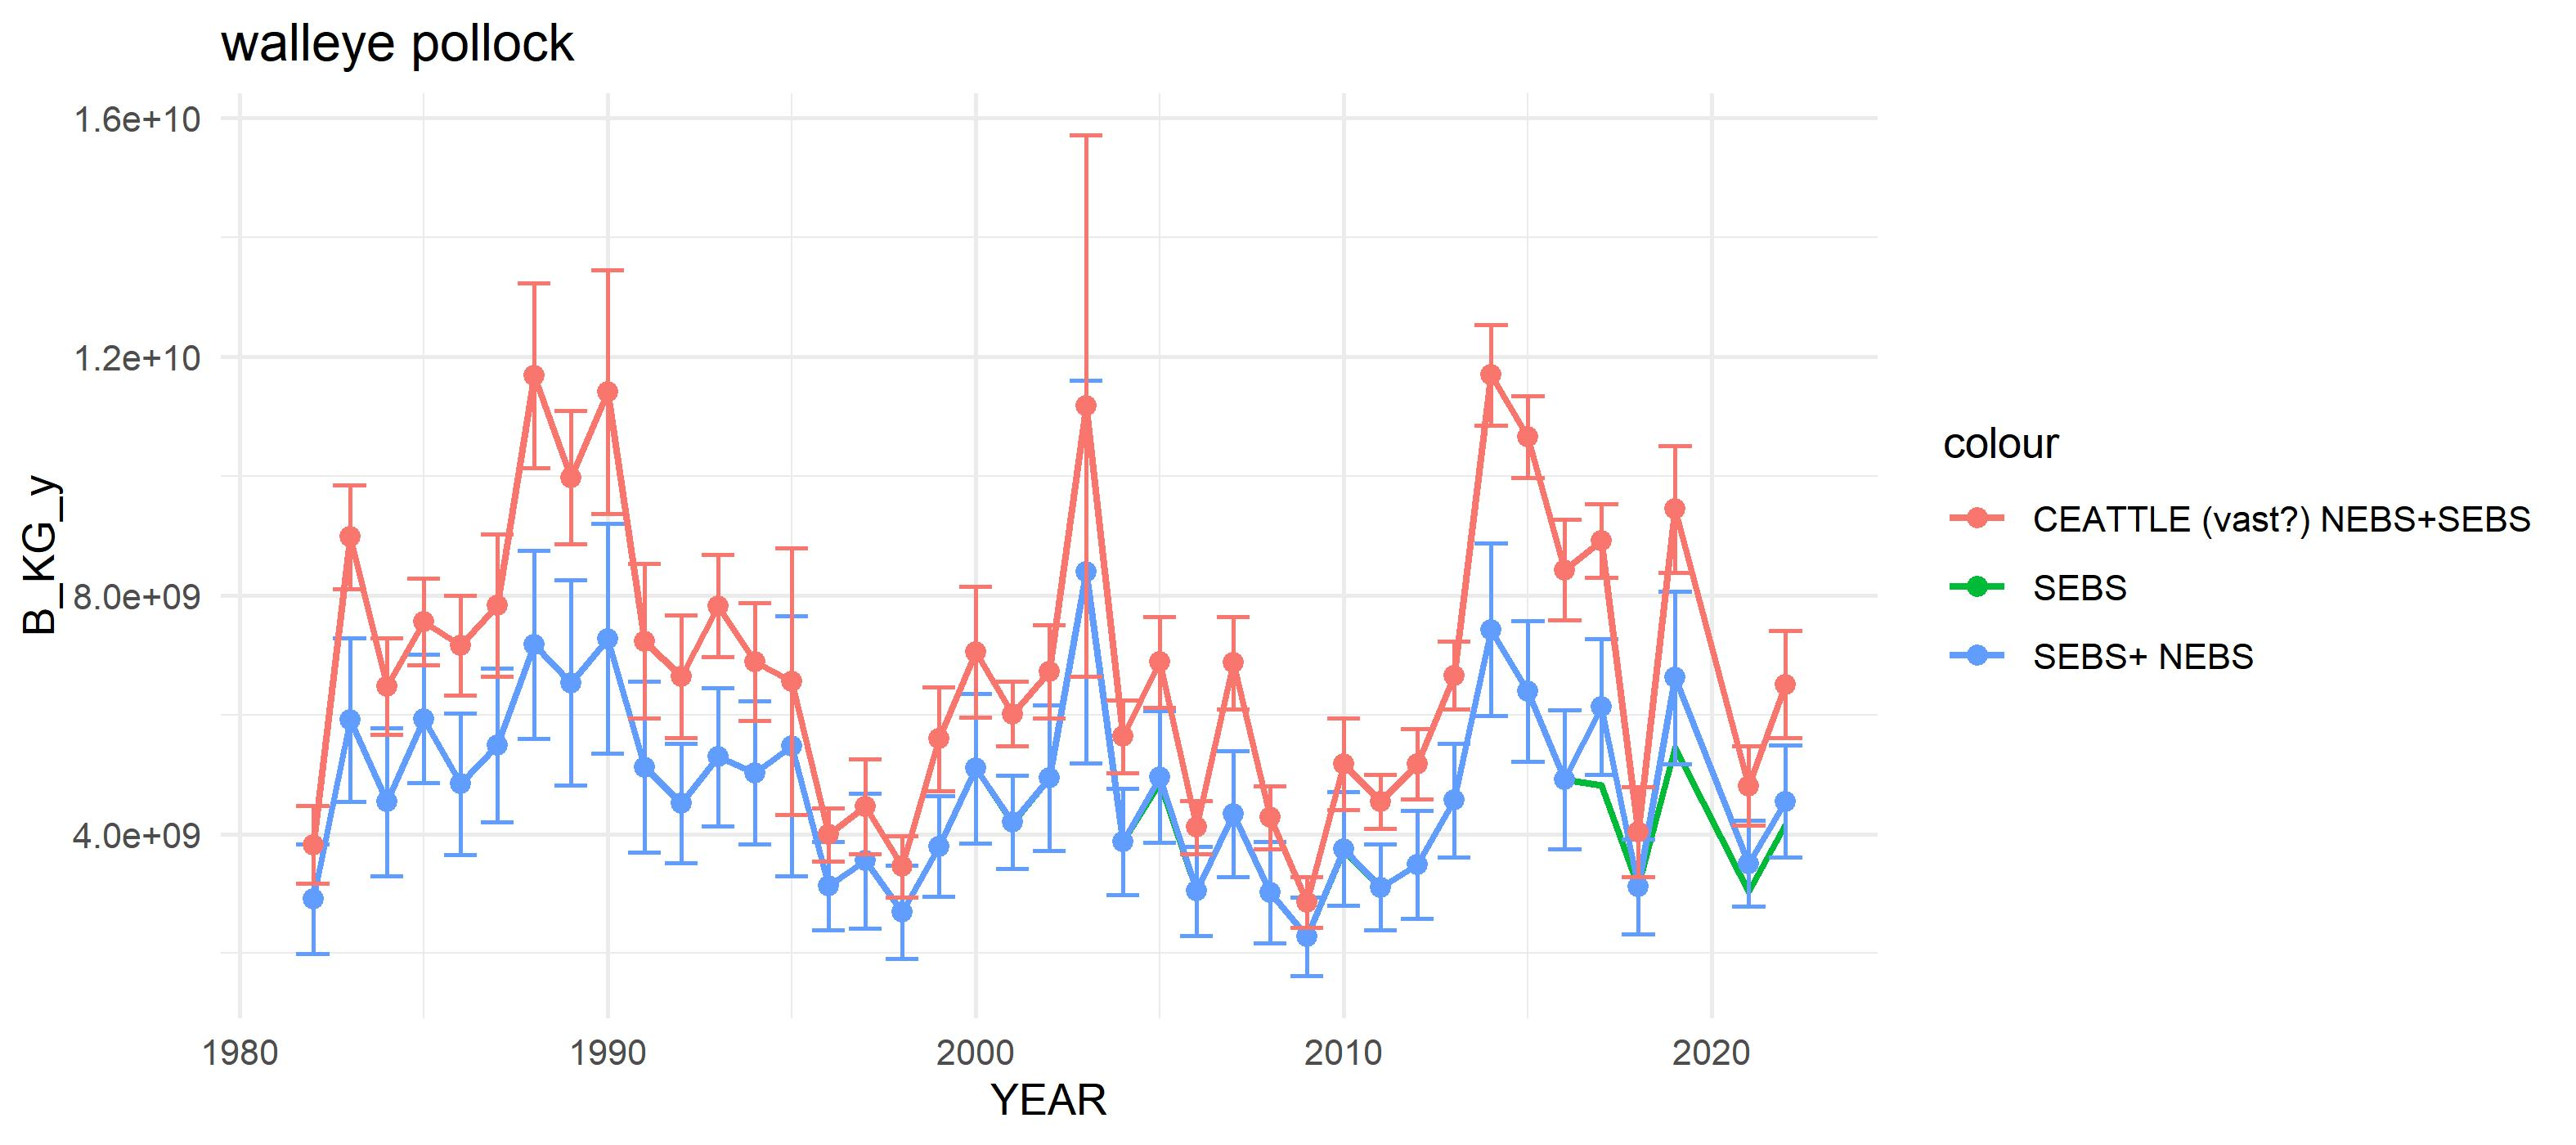
\includegraphics{figs/plk_srvy.jpg}

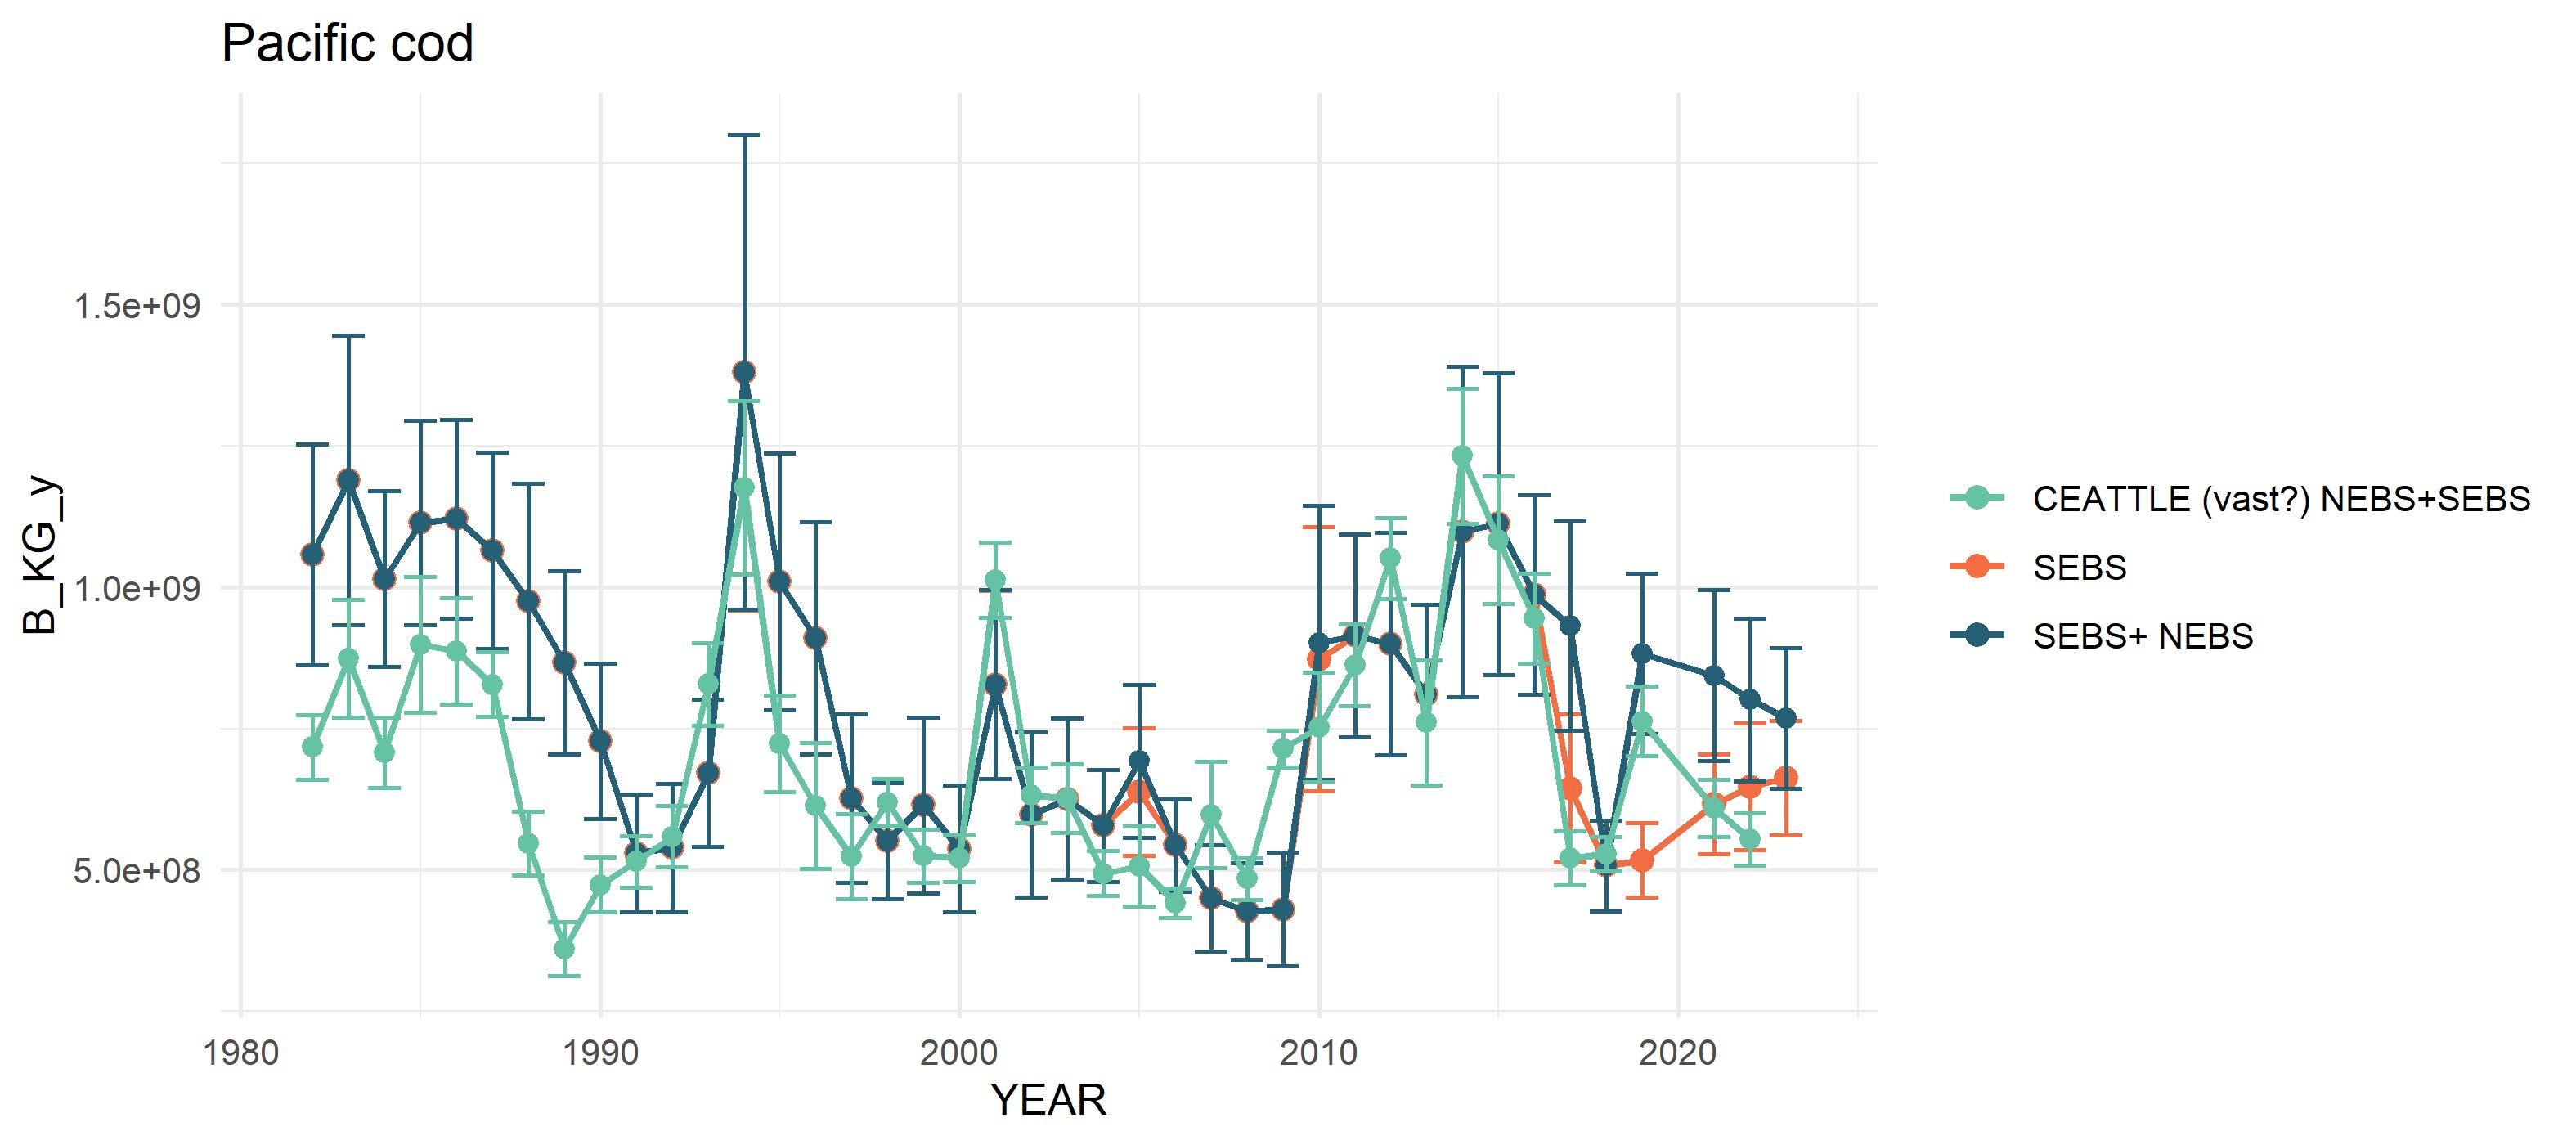
\includegraphics{figs/pcod_srvy.jpg}

\begin{figure}
\centering
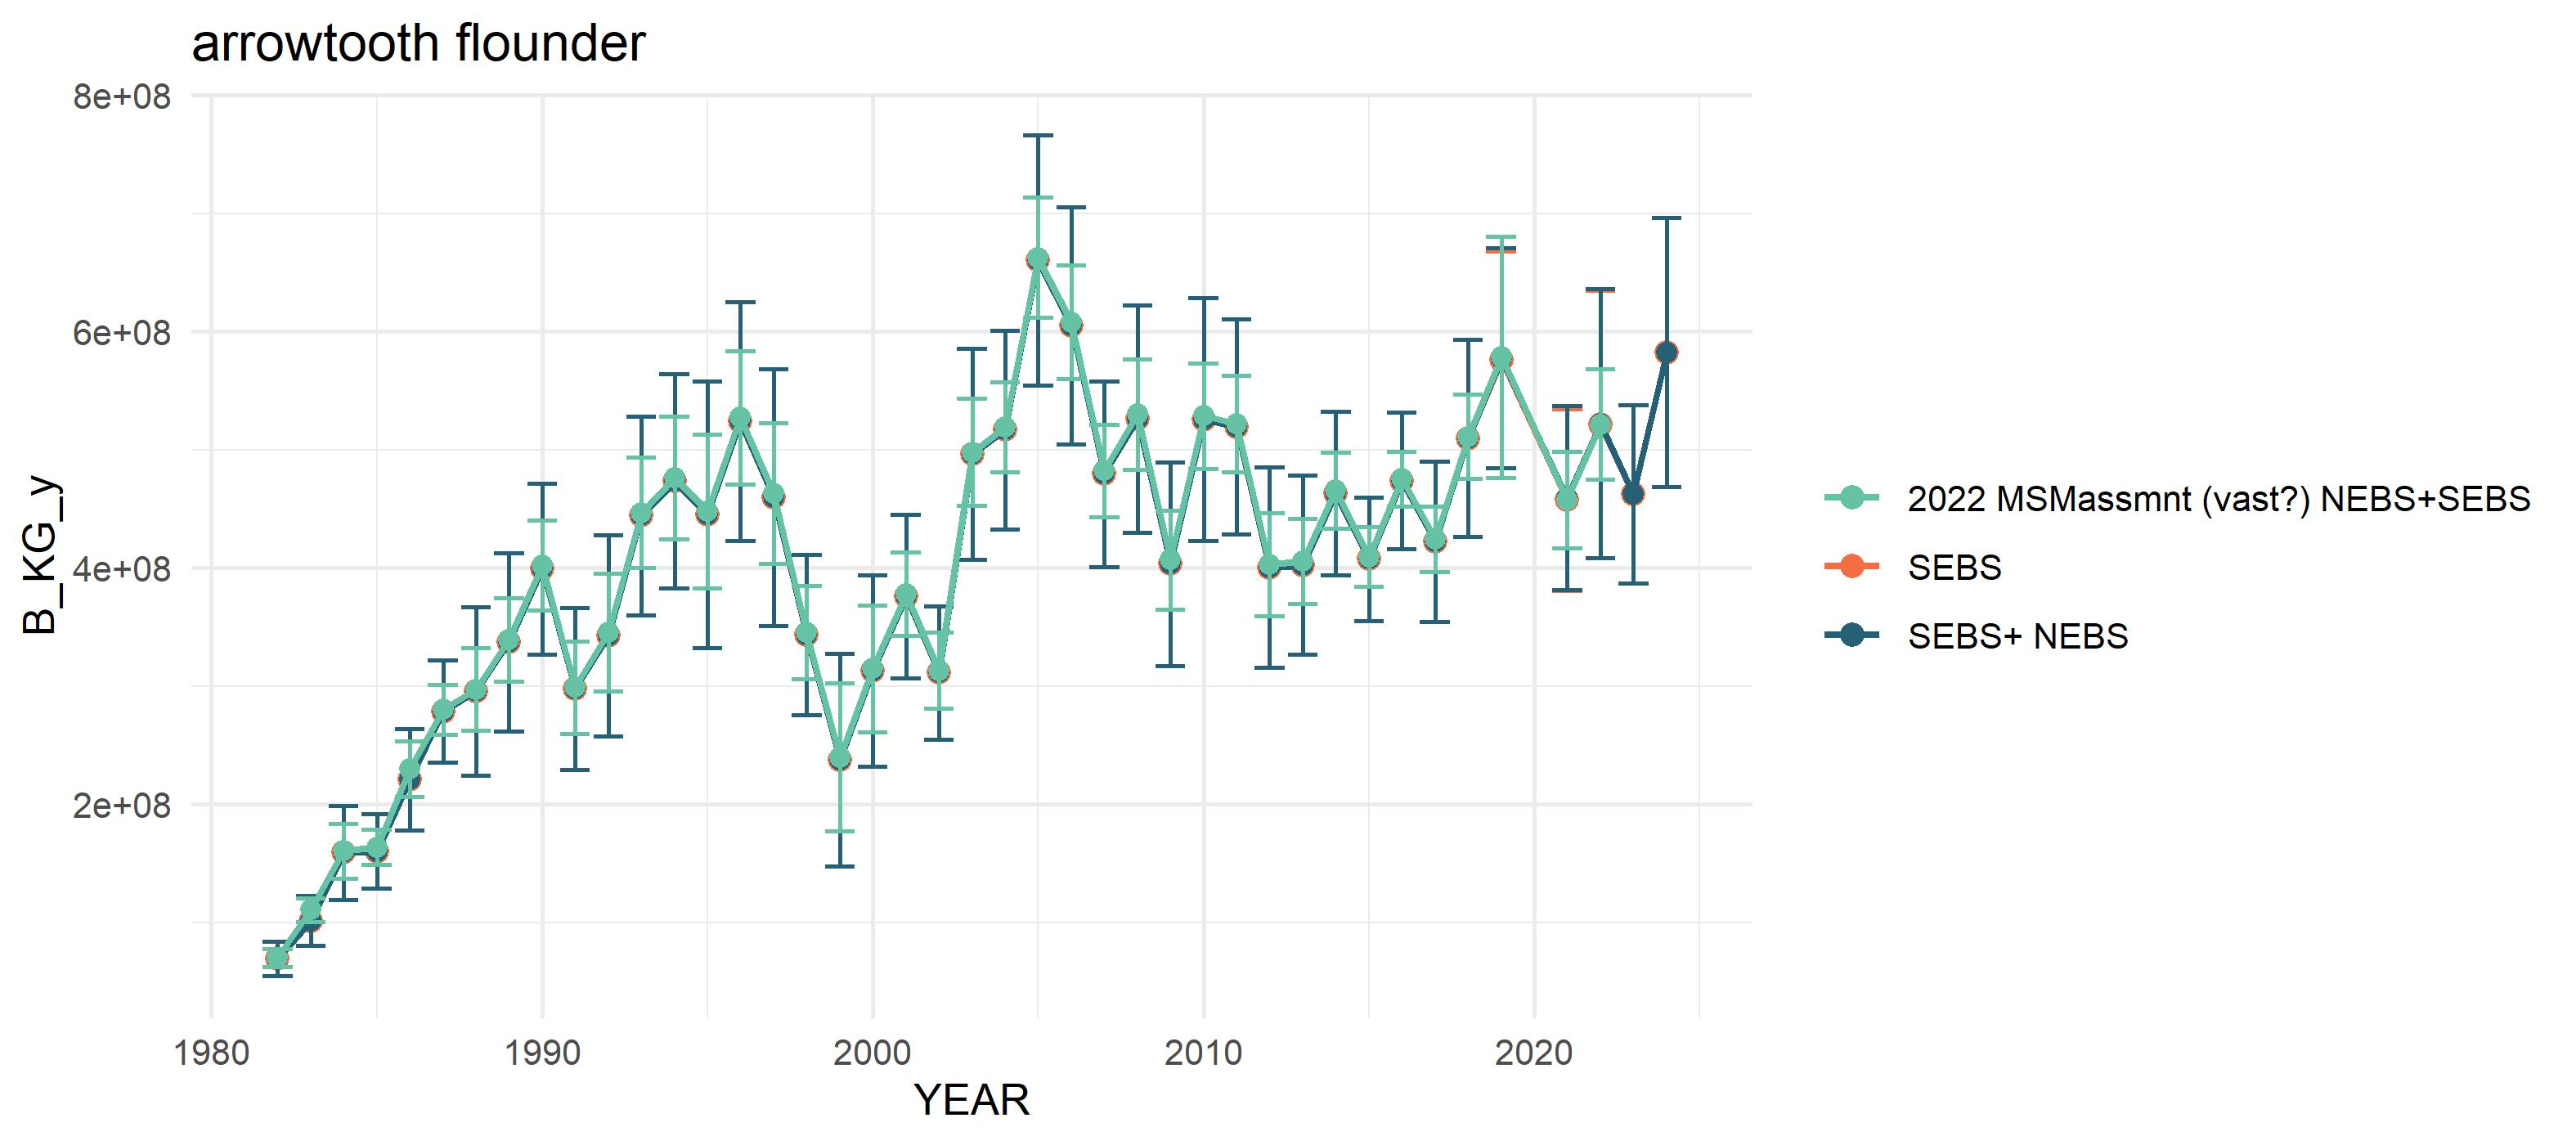
\includegraphics{figs/atf_srvy.jpg}
\caption{``arrowtooth''}
\end{figure}

\hypertarget{code}{%
\section{Code}\label{code}}

\begin{Shaded}
\begin{Highlighting}[]
\CommentTok{\# \#\# Step 0: Set up the R workspace}
\CommentTok{\# }
\CommentTok{\# The first step is to set up the switches for what files to update and create in the file \textasciigrave{}R/setup.R\textasciigrave{}. The code below then loads these settings as well as base data, functions, and packages. }
\CommentTok{\# }
\CommentTok{\# \#\# Step 1: Update SQL queries}
\CommentTok{\# This step must be run on a computer that has access to RACEBASE. The code below will generate the base files for steps 2 and 3 below,and will save them in the folder \textasciigrave{}r data.path \textasciigrave{} under subfolders for each region in \textasciigrave{}srvys$reg\textasciigrave{} and each species in \textasciigrave{}splist\textasciigrave{} (see \textasciigrave{}R/setup.R\textasciigrave{} to change these settings).}

\CommentTok{\# **IMPORTANT:**  }
\CommentTok{\#   }
\CommentTok{\#   * **This step  must be connected to the RACEBASE SQL database**}
\CommentTok{\#   }
\CommentTok{\#   * **To change R studio from the default 64 bit to 32 bit go to Tools\textgreater{}Global options and select the 32 bit version of R.**   }
\CommentTok{\#   }
\CommentTok{\#   * **The code will connect to the SQL database using your password and username. Remember to update the \textasciigrave{}username\_path\textasciigrave{} in the first line of the \textasciigrave{}R/setup.R \textasciigrave{} file and corresponding \textasciigrave{}username\textasciigrave{} and \textasciigrave{}password\textasciigrave{} under \textasciigrave{}username\_password.R\textasciigrave{}. A template is available under \textasciigrave{}R/\textasciigrave{}.**}
\CommentTok{\# }
\CommentTok{\# \textless{}!{-}{-} ![Header of \textasciigrave{}setup.R\textasciigrave{} where \textasciigrave{}username\_path\textasciigrave{} can be adjusted. This file also is where species, regions, and bins are specified.](figs/setup.jpg)\{width=80\%\} {-}{-}\textgreater{}}
\CommentTok{\# }
 
  
  \CommentTok{\# get everything set up:}
  \CommentTok{\#{-}{-}{-}{-}{-}{-}{-}{-}{-}{-}{-}{-}{-}{-}{-}{-}{-}{-}{-}{-}{-}{-}{-}{-}{-}{-}{-}{-}{-}{-}{-}{-}{-}{-}{-}{-}{-}{-}{-}{-}}
    \CommentTok{\# rm(list=ls())}
    \CommentTok{\# this uses the password saved in R/password.R}
    \FunctionTok{suppressMessages}\NormalTok{(}\FunctionTok{source}\NormalTok{(}\StringTok{"R/make.R"}\NormalTok{))}

  \CommentTok{\# update the SQL queries}
  \CommentTok{\#{-}{-}{-}{-}{-}{-}{-}{-}{-}{-}{-}{-}{-}{-}{-}{-}{-}{-}{-}{-}{-}{-}{-}{-}{-}{-}{-}{-}{-}{-}{-}{-}{-}{-}{-}{-}{-}{-}{-}{-}{-}{-}{-}{-}{-}  }

  \FunctionTok{source}\NormalTok{(}\FunctionTok{file.path}\NormalTok{(code.path,}\StringTok{"R/sub\_scripts/runRACE\_qrys.R"}\NormalTok{))}

  \CommentTok{\# combine sebs and nebs into one region: ebs}
  \ControlFlowTok{if}\NormalTok{(}\FunctionTok{dir.exists}\NormalTok{(}\FunctionTok{file.path}\NormalTok{(data.path,}\StringTok{"ebs"}\NormalTok{)))}
      \FunctionTok{system}\NormalTok{(}\FunctionTok{paste}\NormalTok{(}\StringTok{"rm {-}r"}\NormalTok{,}\FunctionTok{file.path}\NormalTok{(data.path,}\StringTok{"ebs"}\NormalTok{)))}
    \FunctionTok{dir.create}\NormalTok{(}\FunctionTok{file.path}\NormalTok{(data.path,}\StringTok{"ebs"}\NormalTok{))}
  
  \CommentTok{\# combine files and rename survey area to all of EBS}
  \ControlFlowTok{for}\NormalTok{(sp }\ControlFlowTok{in} \FunctionTok{names}\NormalTok{(splist))\{}
    \ControlFlowTok{if}\NormalTok{(}\FunctionTok{dir.exists}\NormalTok{(}\FunctionTok{file.path}\NormalTok{(data.path,}\StringTok{"ebs"}\NormalTok{,sp)))}
      \FunctionTok{system}\NormalTok{(}\FunctionTok{paste}\NormalTok{(}\StringTok{"rm {-}r"}\NormalTok{,}\FunctionTok{file.path}\NormalTok{(data.path,}\StringTok{"ebs"}\NormalTok{,sp)))}
      \FunctionTok{dir.create}\NormalTok{(}\FunctionTok{file.path}\NormalTok{(data.path,}\StringTok{"ebs"}\NormalTok{,sp))}
    \CommentTok{\#"length.Rdata"         }
    \FunctionTok{load}\NormalTok{(}\FunctionTok{file.path}\NormalTok{(data.path,}\StringTok{"nebs"}\NormalTok{,sp,}\StringTok{"length.Rdata"}\NormalTok{))}
\NormalTok{    length\_nebs }\OtherTok{\textless{}{-}}\NormalTok{ length;}\FunctionTok{rm}\NormalTok{(length)}
    \FunctionTok{load}\NormalTok{(}\FunctionTok{file.path}\NormalTok{(data.path,}\StringTok{"sebs"}\NormalTok{,sp,}\StringTok{"length.Rdata"}\NormalTok{))}
\NormalTok{    length\_sebs }\OtherTok{\textless{}{-}}\NormalTok{ length;}\FunctionTok{rm}\NormalTok{(length)}
\NormalTok{    length}\OtherTok{\textless{}{-}} \FunctionTok{rbind}\NormalTok{(length\_nebs}\SpecialCharTok{\%\textgreater{}\%}
      \FunctionTok{mutate}\NormalTok{(}\AttributeTok{SURVEY\_DEFINITION\_ID\_aka =}\NormalTok{SURVEY\_DEFINITION\_ID,}\AttributeTok{SURVEY\_DEFINITION\_ID =}\DecValTok{98}\NormalTok{),}
\NormalTok{     length\_sebs}\SpecialCharTok{\%\textgreater{}\%}
      \FunctionTok{mutate}\NormalTok{(}\AttributeTok{SURVEY\_DEFINITION\_ID\_aka =}\NormalTok{SURVEY\_DEFINITION\_ID,}\AttributeTok{SURVEY\_DEFINITION\_ID =}\DecValTok{98}\NormalTok{))}
    
    \FunctionTok{save}\NormalTok{(length,}\AttributeTok{file =} \FunctionTok{file.path}\NormalTok{(data.path,}\StringTok{"ebs"}\NormalTok{,sp,}\StringTok{"length.Rdata"}\NormalTok{))}
    \FunctionTok{rm}\NormalTok{(length)}
    
    \CommentTok{\#"location.Rdata"        }
    \FunctionTok{load}\NormalTok{(}\FunctionTok{file.path}\NormalTok{(data.path,}\StringTok{"nebs"}\NormalTok{,sp,}\StringTok{"location.Rdata"}\NormalTok{))}
\NormalTok{    location\_nebs }\OtherTok{\textless{}{-}}\NormalTok{ location;}\FunctionTok{rm}\NormalTok{(location)}
    \FunctionTok{load}\NormalTok{(}\FunctionTok{file.path}\NormalTok{(data.path,}\StringTok{"sebs"}\NormalTok{,sp,}\StringTok{"location.Rdata"}\NormalTok{))}
\NormalTok{    location\_sebs }\OtherTok{\textless{}{-}}\NormalTok{ location;}\FunctionTok{rm}\NormalTok{(location)}
\NormalTok{    location}\OtherTok{\textless{}{-}} \FunctionTok{rbind}\NormalTok{(location\_nebs, location\_sebs)}
    
    \FunctionTok{save}\NormalTok{(location,}\AttributeTok{file =} \FunctionTok{file.path}\NormalTok{(data.path,}\StringTok{"ebs"}\NormalTok{,sp,}\StringTok{"location.Rdata"}\NormalTok{))}
    
    
    \CommentTok{\#"location\_catch.Rdata"}
    \FunctionTok{load}\NormalTok{(}\FunctionTok{file.path}\NormalTok{(data.path,}\StringTok{"nebs"}\NormalTok{,sp,}\StringTok{"location\_catch.Rdata"}\NormalTok{))}
\NormalTok{    location\_catch\_nebs }\OtherTok{\textless{}{-}}\NormalTok{ location\_catch;}\FunctionTok{rm}\NormalTok{(location\_catch)}
    \FunctionTok{load}\NormalTok{(}\FunctionTok{file.path}\NormalTok{(data.path,}\StringTok{"sebs"}\NormalTok{,sp,}\StringTok{"location\_catch.Rdata"}\NormalTok{))}
\NormalTok{    location\_catch\_sebs }\OtherTok{\textless{}{-}}\NormalTok{ location\_catch;}\FunctionTok{rm}\NormalTok{(location\_catch)}
\NormalTok{    location\_catch }\OtherTok{\textless{}{-}} \FunctionTok{rbind}\NormalTok{(location\_catch\_nebs}\SpecialCharTok{\%\textgreater{}\%}
      \FunctionTok{mutate}\NormalTok{(}\AttributeTok{SURVEY\_DEFINITION\_ID\_aka =}\NormalTok{SURVEY\_DEFINITION\_ID,}\AttributeTok{SURVEY\_DEFINITION\_ID =}\DecValTok{98}\NormalTok{),}
\NormalTok{     location\_catch\_sebs}\SpecialCharTok{\%\textgreater{}\%}
      \FunctionTok{mutate}\NormalTok{(}\AttributeTok{SURVEY\_DEFINITION\_ID\_aka =}\NormalTok{SURVEY\_DEFINITION\_ID,}\AttributeTok{SURVEY\_DEFINITION\_ID =}\DecValTok{98}\NormalTok{))}
    
    \FunctionTok{save}\NormalTok{(location\_catch,}\AttributeTok{file =} \FunctionTok{file.path}\NormalTok{(data.path,}\StringTok{"ebs"}\NormalTok{,sp,}\StringTok{"location\_catch.Rdata"}\NormalTok{))}
    
\NormalTok{  \}}

    
\CommentTok{\#\textasciigrave{}\textasciigrave{}\textasciigrave{}}


\DocumentationTok{\#\# Step 2: Update the LWA regressions}

\CommentTok{\# The default code for RACEBASE uses set LW relationships, however we prefer to update the LW regressions using glms. Depending on how many observations exist the LW relationships can be region specific or use data across all regions.The default below is all regions combined. This code generates two outputs in \textasciigrave{}r data.out\textasciigrave{}, \textasciigrave{}r LWname\textasciigrave{} and \textasciigrave{}LW\_SmryTable.Rdata\textasciigrave{}. It also updates the \textasciigrave{}species\_lkup$LW\_a\textasciigrave{} and species\_lkup$LW\_b\textasciigrave{} parms used in Step 3.}
\CommentTok{\# }
\CommentTok{\# \#\textasciigrave{}\textasciigrave{}\textasciigrave{}\{r updateLWglms, echo=TRUE, eval=FALSE\}    }

  \CommentTok{\# update the LW regressions }
  \CommentTok{\#{-}{-}{-}{-}{-}{-}{-}{-}{-}{-}{-}{-}{-}{-}{-}{-}{-}{-}{-}{-}{-}{-}{-}{-}{-}{-}{-}{-}{-}{-}{-}{-}{-}{-}{-}{-}{-}{-}{-}{-}{-}{-}{-}{-}{-}  }

  \ControlFlowTok{if}\NormalTok{(update\_LWdata)\{    }
     \FunctionTok{source}\NormalTok{(}\FunctionTok{file.path}\NormalTok{(code.path,}\StringTok{"R/sub\_scripts/updateLW.R"}\NormalTok{))}
     \CommentTok{\# reload with updated data:}
     \FunctionTok{source}\NormalTok{(}\FunctionTok{file.path}\NormalTok{(code.path,}\StringTok{"R/load\_data.R"}\NormalTok{))}
\NormalTok{  \}}
\NormalTok{  species\_lkup}

\CommentTok{\#\textasciigrave{}\textasciigrave{}\textasciigrave{}}


\DocumentationTok{\#\# Step 3: Get CPUE data from the surveys}

\CommentTok{\#This code is the core script for generating the CPUE\_NUMKM2 and CPUE\_BIOMKM2 values by size bin, region, and species. }

\CommentTok{\#\textasciigrave{}\textasciigrave{}\textasciigrave{}\{r updateCPUE, echo=TRUE, eval=FALSE\} }
  
\NormalTok{  STRATA\_AREA}\SpecialCharTok{\%\textgreater{}\%}\FunctionTok{filter}\NormalTok{(REGION}\SpecialCharTok{==}\StringTok{"BS"}\NormalTok{)}\SpecialCharTok{\%\textgreater{}\%}
    \FunctionTok{group\_by}\NormalTok{(YEAR)}\SpecialCharTok{\%\textgreater{}\%}\FunctionTok{summarise}\NormalTok{(}\AttributeTok{mnAREA  =} \FunctionTok{mean}\NormalTok{(AREA, }\AttributeTok{na.rm=}\NormalTok{T),}
                               \AttributeTok{sumAREA =} \FunctionTok{sum}\NormalTok{(AREA, }\AttributeTok{na.rm=}\NormalTok{T),}
                               \AttributeTok{cnt =} \FunctionTok{length}\NormalTok{(}\FunctionTok{unique}\NormalTok{(STRATUM)))}
  
\NormalTok{   STRATA\_AREA}\SpecialCharTok{\%\textgreater{}\%}\FunctionTok{filter}\NormalTok{(REGION}\SpecialCharTok{==}\StringTok{"GOA"}\NormalTok{)}\SpecialCharTok{\%\textgreater{}\%}
    \FunctionTok{group\_by}\NormalTok{(YEAR)}\SpecialCharTok{\%\textgreater{}\%}\FunctionTok{summarise}\NormalTok{(}\AttributeTok{mnAREA  =} \FunctionTok{mean}\NormalTok{(AREA, }\AttributeTok{na.rm=}\NormalTok{T),}
                               \AttributeTok{sumAREA =} \FunctionTok{sum}\NormalTok{(AREA, }\AttributeTok{na.rm=}\NormalTok{T),}
                               \AttributeTok{cnt =} \FunctionTok{length}\NormalTok{(}\FunctionTok{unique}\NormalTok{(STRATUM)))}
  
\NormalTok{   STRATA\_AREA}\SpecialCharTok{\%\textgreater{}\%}\FunctionTok{filter}\NormalTok{(REGION}\SpecialCharTok{==}\StringTok{"BS"}\NormalTok{,YEAR}\SpecialCharTok{==}\DecValTok{2022}\NormalTok{)}\SpecialCharTok{\%\textgreater{}\%}\FunctionTok{select}\NormalTok{(STRATUM)}

   \CommentTok{\# overwrite the NEBS frame from setup for the next set of code (ebs = sebs+nebs now forward)}
\NormalTok{  srvys }\OtherTok{\textless{}{-}} \FunctionTok{data.frame}\NormalTok{(}\AttributeTok{reg=}\FunctionTok{c}\NormalTok{(}\StringTok{"ebs"}\NormalTok{,}\StringTok{"goa"}\NormalTok{,}\StringTok{"ai"}\NormalTok{,}\StringTok{"slope"}\NormalTok{),}\AttributeTok{RGN =} \FunctionTok{c}\NormalTok{(}\StringTok{"BS"}\NormalTok{,}\StringTok{"GOA"}\NormalTok{,}\StringTok{"AI"}\NormalTok{,}\StringTok{"SLOPE"}\NormalTok{), }\AttributeTok{num=}\FunctionTok{c}\NormalTok{(}\DecValTok{98}\NormalTok{,}\DecValTok{47}\NormalTok{,}\DecValTok{52}\NormalTok{,}\DecValTok{78}\NormalTok{)  )}
  \CommentTok{\# srvys \textless{}{-} data.frame(reg=c("ebs","goa","ai"),RGN = c("BS","GOA","AI"), num=c(98,47,52)  )}
\NormalTok{  nreg }\OtherTok{\textless{}{-}} \FunctionTok{length}\NormalTok{(srvys}\SpecialCharTok{$}\NormalTok{reg)}
\NormalTok{  nspp }\OtherTok{\textless{}{-}} \FunctionTok{length}\NormalTok{(species\_lkup}\SpecialCharTok{$}\NormalTok{sp)}
  
  \ControlFlowTok{for}\NormalTok{ (r }\ControlFlowTok{in} \DecValTok{1}\SpecialCharTok{:}\NormalTok{nreg)\{}
    \ControlFlowTok{for}\NormalTok{(s }\ControlFlowTok{in} \DecValTok{1}\SpecialCharTok{:}\NormalTok{nspp)\{}
      
      \ControlFlowTok{if}\NormalTok{(srvys[r,]}\SpecialCharTok{$}\NormalTok{reg }\SpecialCharTok{==}\StringTok{"ebs"}\NormalTok{)\{}
        \CommentTok{\# first SEBS only:}
        \CommentTok{\# {-}{-}{-}{-}{-}{-}{-}{-}{-}{-}{-}{-}{-}{-}{-}{-}{-}{-}{-}{-}{-}{-}{-}{-}{-}{-}{-}{-}{-}{-}{-}}
\NormalTok{        STRATA\_AREAUSE }\OtherTok{\textless{}{-}}\NormalTok{ STRATA\_AREA}\SpecialCharTok{\%\textgreater{}\%}\FunctionTok{filter}\NormalTok{(REGION}\SpecialCharTok{==}\NormalTok{srvys}\SpecialCharTok{$}\NormalTok{RGN[r])}
\NormalTok{        maxyr }\OtherTok{\textless{}{-}} \FunctionTok{max}\NormalTok{(STRATA\_AREAUSE}\SpecialCharTok{$}\NormalTok{YEAR)}
\NormalTok{        STRATA\_AREAUSE }\OtherTok{\textless{}{-}}\NormalTok{ STRATA\_AREAUSE}\SpecialCharTok{\%\textgreater{}\%}
          \FunctionTok{filter}\NormalTok{(YEAR}\SpecialCharTok{==}\DecValTok{2022}\NormalTok{)}\SpecialCharTok{\%\textgreater{}\%}
          \FunctionTok{group\_by}\NormalTok{(REGION,STRATUM)}\SpecialCharTok{\%\textgreater{}\%}
          \FunctionTok{summarize}\NormalTok{(}\AttributeTok{AREA =} \FunctionTok{mean}\NormalTok{(AREA, }\AttributeTok{na.rm=}\NormalTok{T))}\SpecialCharTok{\%\textgreater{}\%}\FunctionTok{ungroup}\NormalTok{()}
        
\NormalTok{         flnm }\OtherTok{\textless{}{-}} \FunctionTok{paste0}\NormalTok{(}\StringTok{"s"}\NormalTok{,srvys[r,]}\SpecialCharTok{$}\NormalTok{reg,}\StringTok{".srvy"}\NormalTok{,}
\NormalTok{                     srvys[r,]}\SpecialCharTok{$}\NormalTok{num,}\StringTok{"."}\NormalTok{,}
\NormalTok{                     species\_lkup[s,]}\SpecialCharTok{$}\NormalTok{sp)}
        \FunctionTok{cat}\NormalTok{(}\StringTok{"now getting data for: "}\NormalTok{,flnm,}\StringTok{"}\SpecialCharTok{\textbackslash{}n}\StringTok{"}\NormalTok{)}
\NormalTok{        cpue\_data }\OtherTok{\textless{}{-}} \FunctionTok{suppressMessages}\NormalTok{(}
          \FunctionTok{get\_CPUE\_DATA}\NormalTok{(}
          \AttributeTok{datapath   =}\NormalTok{ data.path,}
          \AttributeTok{out\_dir    =} \FunctionTok{file.path}\NormalTok{(data.out),}
          \AttributeTok{STRATA\_AREAIN =}\NormalTok{ STRATA\_AREAUSE,}
          \AttributeTok{flnm       =}\NormalTok{ flnm,}
          \AttributeTok{species    =}\NormalTok{ species\_lkup[s,]}\SpecialCharTok{$}\NormalTok{SPECIES\_CODE,}
          \AttributeTok{survey     =}\NormalTok{ srvys[r,]}\SpecialCharTok{$}\NormalTok{num,}
          \AttributeTok{includeNBS =} \ConstantTok{FALSE}\NormalTok{,}
          \AttributeTok{NEBSStrataIN =}\NormalTok{ NEBS\_strata ,}
          \AttributeTok{saveit     =}\NormalTok{ T,}
          \AttributeTok{bins       =}\NormalTok{ sp\_bins[[ species\_lkup[s,]}\SpecialCharTok{$}\NormalTok{sp ]]))}
        
        \FunctionTok{rm}\NormalTok{(cpue\_data)}
        
        \CommentTok{\# Now NESB + SEBS}
        \CommentTok{\# {-}{-}{-}{-}{-}{-}{-}{-}{-}{-}{-}{-}{-}{-}{-}{-}{-}{-}{-}{-}{-}{-}{-}{-}{-}{-}{-}{-}{-}{-}{-}}
\NormalTok{        flnm }\OtherTok{\textless{}{-}} \FunctionTok{paste0}\NormalTok{(srvys[r,]}\SpecialCharTok{$}\NormalTok{reg,}\StringTok{".srvy"}\NormalTok{,}
\NormalTok{                     srvys[r,]}\SpecialCharTok{$}\NormalTok{num,}\StringTok{"."}\NormalTok{,}
\NormalTok{                     species\_lkup[s,]}\SpecialCharTok{$}\NormalTok{sp)}
        \FunctionTok{cat}\NormalTok{(}\StringTok{"now getting data for: "}\NormalTok{,flnm,}\StringTok{"}\SpecialCharTok{\textbackslash{}n}\StringTok{"}\NormalTok{)}
\NormalTok{        cpue\_data }\OtherTok{\textless{}{-}} \FunctionTok{suppressMessages}\NormalTok{(}
          \FunctionTok{get\_CPUE\_DATA}\NormalTok{(}
          \AttributeTok{datapath   =}\NormalTok{ data.path,}
          \AttributeTok{out\_dir    =} \FunctionTok{file.path}\NormalTok{(data.out),}
          \AttributeTok{STRATA\_AREAIN =}\NormalTok{ STRATA\_AREAUSE,}
          \AttributeTok{flnm       =}\NormalTok{ flnm,}
          \AttributeTok{species    =}\NormalTok{ species\_lkup[s,]}\SpecialCharTok{$}\NormalTok{SPECIES\_CODE,}
          \AttributeTok{survey     =}\NormalTok{ srvys[r,]}\SpecialCharTok{$}\NormalTok{num,}
          \AttributeTok{includeNBS   =} \ConstantTok{TRUE}\NormalTok{,}
          \AttributeTok{NEBSStrataIN =}\NormalTok{ NEBS\_strata ,}
          \AttributeTok{saveit     =}\NormalTok{ T,}
          \AttributeTok{bins       =}\NormalTok{ sp\_bins[[ species\_lkup[s,]}\SpecialCharTok{$}\NormalTok{sp ]]))}
        
\NormalTok{      \}}
      \ControlFlowTok{if}\NormalTok{(srvys[r,]}\SpecialCharTok{$}\NormalTok{reg }\SpecialCharTok{==}\StringTok{"goa"}\NormalTok{)\{}
\NormalTok{        STRATA\_AREAUSE }\OtherTok{\textless{}{-}}\NormalTok{ STRATA\_AREA}\SpecialCharTok{\%\textgreater{}\%}\FunctionTok{filter}\NormalTok{(REGION}\SpecialCharTok{==}\NormalTok{srvys}\SpecialCharTok{$}\NormalTok{RGN[r])}
\NormalTok{        maxyr }\OtherTok{\textless{}{-}} \FunctionTok{max}\NormalTok{(STRATA\_AREAUSE}\SpecialCharTok{$}\NormalTok{YEAR)}
\NormalTok{        STRATA\_AREAUSE }\OtherTok{\textless{}{-}}\NormalTok{ STRATA\_AREAUSE}\SpecialCharTok{\%\textgreater{}\%}
          \FunctionTok{filter}\NormalTok{(YEAR}\SpecialCharTok{==}\DecValTok{1993}\NormalTok{)}\SpecialCharTok{\%\textgreater{}\%}
          \FunctionTok{group\_by}\NormalTok{(REGION,STRATUM)}\SpecialCharTok{\%\textgreater{}\%}
          \FunctionTok{summarize}\NormalTok{(}\AttributeTok{AREA =} \FunctionTok{mean}\NormalTok{(AREA, }\AttributeTok{na.rm=}\NormalTok{T))}\SpecialCharTok{\%\textgreater{}\%}\FunctionTok{ungroup}\NormalTok{()}
        
\NormalTok{        flnm }\OtherTok{\textless{}{-}} \FunctionTok{paste0}\NormalTok{(srvys[r,]}\SpecialCharTok{$}\NormalTok{reg,}\StringTok{".srvy"}\NormalTok{,}
\NormalTok{                     srvys[r,]}\SpecialCharTok{$}\NormalTok{num,}\StringTok{"."}\NormalTok{,}
\NormalTok{                     species\_lkup[s,]}\SpecialCharTok{$}\NormalTok{sp)}
        \FunctionTok{cat}\NormalTok{(}\StringTok{"now getting data for: "}\NormalTok{,flnm,}\StringTok{"}\SpecialCharTok{\textbackslash{}n}\StringTok{"}\NormalTok{)}
\NormalTok{        cpue\_data }\OtherTok{\textless{}{-}} \FunctionTok{suppressMessages}\NormalTok{(}
          \FunctionTok{get\_CPUE\_DATA}\NormalTok{(}
          \AttributeTok{datapath   =}\NormalTok{ data.path,}
          \AttributeTok{out\_dir    =} \FunctionTok{file.path}\NormalTok{(data.out),}
          \AttributeTok{STRATA\_AREAIN =}\NormalTok{ STRATA\_AREAUSE,}
          \AttributeTok{flnm       =}\NormalTok{ flnm,}
          \AttributeTok{species    =}\NormalTok{ species\_lkup[s,]}\SpecialCharTok{$}\NormalTok{SPECIES\_CODE,}
          \AttributeTok{survey     =}\NormalTok{ srvys[r,]}\SpecialCharTok{$}\NormalTok{num,}
          \AttributeTok{includeNBS =} \ConstantTok{FALSE}\NormalTok{,}
          \AttributeTok{NEBSStrataIN =}\NormalTok{ NEBS\_strata ,}
          \AttributeTok{saveit     =}\NormalTok{ T,}
          \AttributeTok{bins       =}\NormalTok{ sp\_bins[[ species\_lkup[s,]}\SpecialCharTok{$}\NormalTok{sp ]]))}
        
\NormalTok{      \}}
      \ControlFlowTok{if}\NormalTok{(}\SpecialCharTok{!}\NormalTok{srvys[r,]}\SpecialCharTok{$}\NormalTok{reg}\SpecialCharTok{\%in\%}\FunctionTok{c}\NormalTok{(}\StringTok{"ebs"}\NormalTok{,}\StringTok{"goa"}\NormalTok{))\{}
\NormalTok{        flnm }\OtherTok{\textless{}{-}} \FunctionTok{paste0}\NormalTok{(srvys[r,]}\SpecialCharTok{$}\NormalTok{reg,}\StringTok{".srvy"}\NormalTok{,}
\NormalTok{                     srvys[r,]}\SpecialCharTok{$}\NormalTok{num,}\StringTok{"."}\NormalTok{,}
\NormalTok{                     species\_lkup[s,]}\SpecialCharTok{$}\NormalTok{sp)}
        \FunctionTok{cat}\NormalTok{(}\StringTok{"now getting data for: "}\NormalTok{,flnm,}\StringTok{"}\SpecialCharTok{\textbackslash{}n}\StringTok{"}\NormalTok{)}
\NormalTok{        cpue\_data }\OtherTok{\textless{}{-}} \FunctionTok{suppressMessages}\NormalTok{(}
          \FunctionTok{get\_CPUE\_DATA}\NormalTok{(}
          \AttributeTok{datapath   =}\NormalTok{ data.path,}
          \AttributeTok{out\_dir    =} \FunctionTok{file.path}\NormalTok{(data.out),}
          \AttributeTok{STRATA\_AREAIN =} \ConstantTok{NULL}\NormalTok{,}
          \AttributeTok{flnm       =}\NormalTok{ flnm,}
          \AttributeTok{species    =}\NormalTok{ species\_lkup[s,]}\SpecialCharTok{$}\NormalTok{SPECIES\_CODE,}
          \AttributeTok{survey     =}\NormalTok{ srvys[r,]}\SpecialCharTok{$}\NormalTok{num,}
          \AttributeTok{includeNBS =} \ConstantTok{FALSE}\NormalTok{,}
          \AttributeTok{NEBSStrataIN =}\NormalTok{ NEBS\_strata ,}
          \AttributeTok{saveit     =}\NormalTok{ T,}
          \AttributeTok{bins       =}\NormalTok{ sp\_bins[[ species\_lkup[s,]}\SpecialCharTok{$}\NormalTok{sp ]]))}

\NormalTok{      \}}
     
      \CommentTok{\# \# check the data :}
      \ControlFlowTok{if}\NormalTok{(}\DecValTok{1}\SpecialCharTok{==}\DecValTok{10}\NormalTok{)\{}
\NormalTok{        tt }\OtherTok{\textless{}{-}}\NormalTok{ cpue\_data}\SpecialCharTok{\%\textgreater{}\%}
              \FunctionTok{group\_by}\NormalTok{(YEAR,REGION,STATIONID,SN)}\SpecialCharTok{\%\textgreater{}\%}
              \FunctionTok{filter}\NormalTok{(BIN }\SpecialCharTok{==}\DecValTok{400}\NormalTok{)}\SpecialCharTok{\%\textgreater{}\%}
              \FunctionTok{summarize}\NormalTok{(}\AttributeTok{cnt =}\FunctionTok{length}\NormalTok{(STATIONID))}
         \FunctionTok{max}\NormalTok{(tt}\SpecialCharTok{$}\NormalTok{cnt)  }\CommentTok{\#Should be 1}
        \CommentTok{\#this looks to be a duplicate sampling...}
        \CommentTok{\#mis{-}entry or code error ?}
\NormalTok{         cpue\_data}\SpecialCharTok{\%\textgreater{}\%}\FunctionTok{filter}\NormalTok{(YEAR}\SpecialCharTok{==}\DecValTok{1988}\NormalTok{,STATIONID}\SpecialCharTok{==}\StringTok{"J{-}13"}\NormalTok{)}
\NormalTok{      \}}
       \FunctionTok{rm}\NormalTok{(cpue\_data)}

\NormalTok{    \}}
\NormalTok{  \}}
\CommentTok{\#   }
\CommentTok{\# \textasciigrave{}\textasciigrave{}\textasciigrave{}}
\CommentTok{\# }
\CommentTok{\# *The cpue files are now saved in the directory \textasciigrave{}r file.path(data.out,"../")\textasciigrave{}*}
\CommentTok{\# }
\CommentTok{\# \textasciigrave{}\textasciigrave{}\textasciigrave{}\{r viewcpue\_data, echo=TRUE, eval=FALSE\} }
  \CommentTok{\# this uses the password saved in R/password.R}
  \CommentTok{\#  suppressMessages(source("R/make.R"))}
\FunctionTok{load}\NormalTok{(}\FunctionTok{file.path}\NormalTok{(data.out,}\StringTok{"cpue/ebs/ebs.srvy98.pcod.cpue\_data.Rdata"}\NormalTok{))}

\FunctionTok{names}\NormalTok{(cpue\_data)}

\FunctionTok{library}\NormalTok{(dplyr)}

\NormalTok{checkit }\OtherTok{\textless{}{-}}\ControlFlowTok{function}\NormalTok{(x)\{}
   \ControlFlowTok{if}\NormalTok{(}\FunctionTok{round}\NormalTok{(}\FunctionTok{max}\NormalTok{(x ),}\DecValTok{1}\NormalTok{)}\SpecialCharTok{!=}\DecValTok{1}\NormalTok{) \{}
     \FunctionTok{warning}\NormalTok{(}\StringTok{"ERROR! propB \textgreater{} 1 "}\NormalTok{)}
     \FunctionTok{print}\NormalTok{(x)\}}
  
\NormalTok{\}}

  \CommentTok{\#double check the results}
\NormalTok{  cnt\_ByStrataBin }\OtherTok{\textless{}{-}}\NormalTok{ cpue\_data}\SpecialCharTok{$}\NormalTok{propByStrataBin}\SpecialCharTok{\%\textgreater{}\%}
    \FunctionTok{select}\NormalTok{(}\StringTok{"REGION"}\NormalTok{,}\StringTok{"YEAR"}\NormalTok{,}\StringTok{"STRATUM"}\NormalTok{,BIN,BIN\_mm,}
\NormalTok{           SPECIES\_CODE,CN,SN,sp,num,}
           \StringTok{"propB\_ykl"}\NormalTok{,}\StringTok{"propN\_ykl"}\NormalTok{)}\SpecialCharTok{\%\textgreater{}\%}
    \FunctionTok{group\_by}\NormalTok{(YEAR,REGION,SN,CN)}\SpecialCharTok{\%\textgreater{}\%}
    \FunctionTok{summarise}\NormalTok{(}\AttributeTok{sum\_propB\_ykl=}\FunctionTok{sum}\NormalTok{(propB\_ykl,}\AttributeTok{na.rm=}\NormalTok{T),}
              \AttributeTok{sum\_propN\_ykl=}\FunctionTok{sum}\NormalTok{(propN\_ykl,}\AttributeTok{na.rm=}\NormalTok{T))}
  
\NormalTok{  cnt\_ByStrata }\OtherTok{\textless{}{-}}\NormalTok{ cpue\_data}\SpecialCharTok{$}\NormalTok{propByStrata}\SpecialCharTok{\%\textgreater{}\%}
    \FunctionTok{select}\NormalTok{(}\StringTok{"REGION"}\NormalTok{,}\StringTok{"YEAR"}\NormalTok{,}\StringTok{"STRATUM"}\NormalTok{,}
\NormalTok{           SPECIES\_CODE,CN,SN,sp,num,}
           \StringTok{"propB\_yk"}\NormalTok{,}\StringTok{"propN\_yk"}\NormalTok{)}\SpecialCharTok{\%\textgreater{}\%}
    \FunctionTok{group\_by}\NormalTok{(YEAR,REGION,SN,CN)}\SpecialCharTok{\%\textgreater{}\%}
    \FunctionTok{summarise}\NormalTok{(}\AttributeTok{sum\_propB\_yk=}\FunctionTok{sum}\NormalTok{(propB\_yk,}\AttributeTok{na.rm=}\NormalTok{T),}
              \AttributeTok{sum\_propN\_yk=}\FunctionTok{sum}\NormalTok{(propN\_yk,}\AttributeTok{na.rm=}\NormalTok{T))}
    
\NormalTok{  cnt\_ByBin }\OtherTok{\textless{}{-}}\NormalTok{ cpue\_data}\SpecialCharTok{$}\NormalTok{propByBin}\SpecialCharTok{\%\textgreater{}\%}
    \FunctionTok{select}\NormalTok{(}\StringTok{"REGION"}\NormalTok{,}\StringTok{"YEAR"}\NormalTok{,BIN,BIN\_mm,num,}
\NormalTok{           SPECIES\_CODE,CN,SN,sp,}
           \StringTok{"propB\_yl"}\NormalTok{,}\StringTok{"propN\_yl"}\NormalTok{)}\SpecialCharTok{\%\textgreater{}\%}
    \FunctionTok{group\_by}\NormalTok{(YEAR,REGION,SN,CN)}\SpecialCharTok{\%\textgreater{}\%}
    \FunctionTok{summarise}\NormalTok{(}\AttributeTok{sum\_propB\_yl=}\FunctionTok{sum}\NormalTok{(propB\_yl ,}\AttributeTok{na.rm=}\NormalTok{T),}
              \AttributeTok{sum\_propN\_yl=}\FunctionTok{sum}\NormalTok{(propN\_yl ,}\AttributeTok{na.rm=}\NormalTok{T))}
  
  \FunctionTok{checkit}\NormalTok{(cnt\_ByStrataBin}\SpecialCharTok{$}\NormalTok{sum\_propB\_ykl)}
  \FunctionTok{checkit}\NormalTok{(cnt\_ByStrata}\SpecialCharTok{$}\NormalTok{sum\_propB\_yk)}
  \FunctionTok{checkit}\NormalTok{(cnt\_ByBin}\SpecialCharTok{$}\NormalTok{sum\_propB\_yl)}
  
\CommentTok{\# }
\end{Highlighting}
\end{Shaded}

\hypertarget{appendix-1-rsetup.rprimary-setup-script}{%
\subsection{\texorpdfstring{Appendix 1: \texttt{R/setup.R}primary setup
script}{Appendix 1: R/setup.Rprimary setup script}}\label{appendix-1-rsetup.rprimary-setup-script}}

\end{document}
